
\documentclass[modern]{aastex62}
%linenumbers

%\documentclass[DM,authoryear,toc]{lsstdoc}
\newcommand{\docRef}{set the Reference with {$\backslash$}setDocRef}
\newcommand{\setDocRef}[1]{
   \renewcommand{\docRef}{#1}
}

\setDocRef{DMTN-115}
\usepackage{newtxtext,newtxmath} % this is causing the etoolbox warning
\usepackage[USenglish]{babel}
\usepackage[utf8]{inputenc}
\usepackage[T1]{fontenc}
\usepackage{comment}
\usepackage{enumitem}
\usepackage{glossaries}
\usepackage{todonotes}
\usepackage{collect}
\usepackage{wrapfig}

\setlist{noitemsep}

\graphicspath{{./}{./figures/}{./images}}



% Add your own macros here:

\newcommand{\Comment}[3]{\textcolor{#1}{(#2: #3)}}
\newcommand{\AMS}[1]{\Comment{red}{AMS}{#1}} % Arfon Smith's comments

% lsstdoc documentation: https://lsst-texmf.lsst.io/lsstdoc.html

\providecommand{\secref}[1]{Section~\ref{#1}}
\providecommand{\appref}[1]{Appendix~\ref{#1}}
\providecommand{\tabref}[1]{Table~\ref{#1}}
\providecommand{\figref}[1]{Figure~\ref{#1}}
\providecommand{\eqnref}[1]{Eq.~\ref{#1}}
\providecommand{\recref}[1]{REC-\ref{#1}}


% DO NOT EDIT - generated by /Users/womullan/LSSTgit/lsst-texmf/bin/generateAcronyms.py from https://lsst-texmf.lsst.io/.
\newacronym{API} {API} {Application Programming Interface}
\newglossaryentry{AURA} {name={AURA}, description={\gls{Association of Universities for Research in Astronomy}}}
\newacronym{AWS} {AWS} {Amazon Web Services}
\newglossaryentry{Archive} {name={Archive}, description={The repository for documents required by the NSF to be kept. These include documents related to design and development, construction, integration, test, and operations of the LSST observatory system. The archive is maintained using the enterprise content management system DocuShare, which is accessible through a link on the project website www.project.lsst.org.}}
\newglossaryentry{Archive Center} {name={Archive Center}, description={Part of the LSST Data Management System, the LSST archive center is a data center at NCSA that hosts the LSST Archive, which includes released science data and metadata, observatory and engineering data, and supporting software such as the LSST Software Stack.}}
\newglossaryentry{Association of Universities for Research in Astronomy} {name={Association of Universities for Research in Astronomy}, description={ consortium of US institutions and international affiliates that operates world-class astronomical observatories, AURA is the legal entity responsible for managing what it calls independent operating Centers, including LSST, under respective cooperative agreements with the National Science Foundation. AURA assumes fiducial responsibility for the funds provided through those cooperative agreements. AURA also is the legal owner of the AURA Observatory properties in Chile.}}
\newglossaryentry{Butler} {name={Butler}, description={A middleware component for persisting and retrieving image datasets (raw or processed), calibration reference data, and catalogs.}}
\newacronym{CAOM} {CAOM} {Common Archive Observation Model}
\newglossaryentry{CRUD} {name={CRUD}, description={Create Retrieve Update and Destroy}}
\newacronym{CSV} {CSV} {Comma Separated Values}
\newglossaryentry{Center} {name={Center}, description={An entity managed by AURA that is responsible for execution of a federally funded project}}
\newacronym{DM} {DM} {\gls{Data Management}}
\newacronym{DMS} {DMS} {Data Management Subsystem}
\newglossaryentry{DMTN} {name={DMTN}, description={DM Technical Note}}
\newacronym{DR} {DR} {Data Release}
\newacronym{DRP} {DRP} {Data Release Production}
\newglossaryentry{Data Management} {name={Data Management}, description={The LSST Subsystem responsible for the Data Management System (DMS), which will capture, store, catalog, and serve the LSST dataset to the scientific community and public. The DM team is responsible for the DMS architecture, applications, middleware, infrastructure, algorithms, and Observatory Network Design. DM is a distributed team working at LSST and partner institutions, with the DM Subsystem Manager located at LSST headquarters in Tucson.}}
\newglossaryentry{Data Management Subsystem} {name={Data Management Subsystem}, description={The subsystems within Data Management may contain a defined combination of hardware, a software stack, a set of running processes, and the people who manage them: they are a major component of the DM System operations. Examples include the 'Archive Operations Subsystem' and the 'Data Processing Subsystem'"."}}
\newglossaryentry{Data Management System} {name={Data Management System}, description={The computing infrastructure, middleware, and applications that process, store, and enable information extraction from the LSST dataset; the DMS will process peta-scale data volume, convert raw images into a faithful representation of the universe, and archive the results in a useful form. The infrastructure layer consists of the computing, storage, networking hardware, and system software. The middleware layer handles distributed processing, data access, user interface, and system operations services. The applications layer includes the data pipelines and the science data archives' products and services.}}
\newglossaryentry{Data Release} {name={Data Release}, description={The approximately annual reprocessing of all LSST data, and the installation of the resulting data products in the LSST Data Access Centers, which marks the start of the two-year proprietary period.}}
\newglossaryentry{Data Release Production} {name={Data Release Production}, description={An episode of (re)processing all of the accumulated LSST images, during which all output DR data products are generated. These episodes are planned to occur annually during the LSST survey, and the processing will be executed at the Archive Center. This includes Difference Imaging Analysis, generating deep Coadd Images, Source detection and association, creating Object and Solar System Object catalogs, and related metadata.}}
\newglossaryentry{DocuShare} {name={DocuShare}, description={The trade name for the enterprise management software used by LSST to archive and manage documents}}
\newacronym{FITS} {FITS} {\gls{Flexible Image Transport System}}
\newglossaryentry{FSAAS} {name={FSAAS}, description={Filesystem as a Service}}
\newglossaryentry{FUSE} {name={FUSE}, description={a user space filesystem framework}}
\newglossaryentry{Flexible Image Transport System} {name={Flexible Image Transport System}, description={an international standard in astronomy for storing images, tables, and metadata in disk files. See the IAU FITS Standard for details.}}
\newacronym{HDF} {HDF} {Hierarchical Data Format}
\newacronym{HPC} {HPC} {High Performance Computing}
\newacronym{HTC} {HTC} {High Throughput Computing}
\newacronym{IAU} {IAU} {International Astronomical Union}
\newglossaryentry{IRAF} {name={IRAF}, description={Image Reduction and Analysis Facility}}
\newglossaryentry{JSON} {name={JSON}, description={JavaScript Object Notation}}
\newacronym{LSST} {LSST} {Large Synoptic Survey Telescope}
\newglossaryentry{NCSA} {name={NCSA}, description={National Center for Supercomputing Applications}}
\newacronym{NSF} {NSF} {\gls{National Science Foundation}}
\newglossaryentry{National Science Foundation} {name={National Science Foundation}, description={primary federal agency supporting research in all fields of fundamental science and engineering; NSF selects and funds projects through competitive, merit-based review}}
\newglossaryentry{Object} {name={Object}, description={In LSST nomenclature this refers to an astronomical object, such as a star, galaxy, or other physical entity. E.g., comets, asteroids are also Objects but typically called a Moving Object or a Solar System Object (SSObject). One of the DRP data products is a table of Objects detected by LSST which can be static, or change brightness or position with time.}}
\newglossaryentry{Operations} {name={Operations}, description={The 10-year period following construction and commissioning during which the LSST Observatory conducts its survey}}
\newglossaryentry{POSIX} {name={POSIX}, description={Portable Operating System Interface}}
\newglossaryentry{Project Manager} {name={Project Manager}, description={The person responsible for exercising leadership and oversight over the entire LSST project; he or she controls schedule, budget, and all contingency funds}}
\newglossaryentry{Science Pipelines} {name={Science Pipelines}, description={The library of software components and the algorithms and processing pipelines assembled from them that are being developed by DM to generate science-ready data products from LSST images. The Pipelines may be executed at scale as part of LSST Prompt or Data Release processing, or pieces of them may be used in a standalone mode or executed through the LSST Science Platform. The Science Pipelines are one component of the LSST Software Stack.}}
\newglossaryentry{Science Platform} {name={Science Platform}, description={A set of integrated web applications and services deployed at the LSST Data Access Centers (DACs) through which the scientific community will access, visualize, and perform next-to-the-data analysis of the LSST data products.}}
\newglossaryentry{Software Stack} {name={Software Stack}, description={Often referred to as the LSST Stack, or just The Stack, it is the collection of software written by the LSST Data Management Team to process, generate, and serve LSST images, transient alerts, and catalogs. The Stack includes the LSST Science Pipelines, as well as packages upon which the DM software depends. It is open source and publicly available.}}
\newglossaryentry{Solar System Object} {name={Solar System Object}, description={A solar system object is an astrophysical object that is identified as part of the Solar System: planets and their satellites, asteroids, comets, etc. This class of object had historically been referred to within the LSST Project as Moving Objects.}}
\newglossaryentry{Source} {name={Source}, description={A single detection of an astrophysical object in an image, the characteristics for which are stored in the Source Catalog of the DRP database. The association of Sources that are non-moving lead to Objects; the association of moving Sources leads to Solar System Objects. (Note that in non-LSST usage "source" is often used for what LSST calls an Object.)}}
\newglossaryentry{Subsystem} {name={Subsystem}, description={A set of elements comprising a system within the larger LSST system that is responsible for a key technical deliverable of the project.}}
\newglossaryentry{Subsystem Manager} {name={Subsystem Manager}, description={responsible manager for an LSST subsystem; he or she exercises authority, within prescribed limits and under scrutiny of the Project Manager, over the relevant subsystem's cost, schedule, and work plans}}
\newacronym{US} {US} {United States}
\newacronym{VO} {VO} {Virtual Observatory}
\newglossaryentry{astronomical object} {name={astronomical object}, description={A star, galaxy, asteroid, or other physical object of astronomical interest. Beware: in non-LSST usage, these are often known as sources.}}
\newglossaryentry{calibration} {name={calibration}, description={The process of translating signals produced by a measuring instrument such as a telescope and camera into physical units such as flux, which are used for scientific analysis. Calibration removes most of the contributions to the signal from environmental and instrumental factors, such that only the astronomical component remains.}}
\newglossaryentry{camera} {name={camera}, description={An imaging device mounted at a telescope focal plane, composed of optics, a shutter, a set of filters, and one or more sensors arranged in a focal plane array.}}
\newglossaryentry{flux} {name={flux}, description={Shorthand for radiative flux, it is a measure of the transport of radiant energy per unit area per unit time. In astronomy this is usually expressed in cgs units: erg/cm2/s.}}
\newglossaryentry{metadata} {name={metadata}, description={General term for data about data, e.g., attributes of astronomical objects (e.g. images, sources, astroObjects, etc.) that are characteristics of the objects themselves, and facilitate the organization, preservation, and query of data sets. (E.g., a FITS header contains metadata).}}
\newglossaryentry{stack} {name={stack}, description={A record of all versions of a document uploaded to a particular DocuShare handle}}
\newglossaryentry{transient} {name={transient}, description={A transient source is one that has been detected on a difference image, but has not been associated with either an astronomical object or a solar system body.}}

\makeglossaries

\begin{document}



\author{William~O'Mullane.}
\affiliation{Large Synoptic Survey Telescope (LSST/AURA)}
\author{Niall~Gaffney}
\affiliation{Texas Advanced Computing Center}
\author{Frossie~Economou}
\affiliation{Large Synoptic Survey Telescope (LSST/AURA)}
\author{Arfon~M.~Smith}
\affiliation{Space Telescope Science Institute}
\author{J.~Ross~Thomson}
\affiliation{Google}
\author{Tim~Jenness}
\affiliation{Large Synoptic Survey Telescope (LSST/AURA)}

\date{\today}

\keywords{Astronomy, Astrophysics, Data Management, Computing, HPC, HTC, Networking, Cloud, Files   }
%should be 350 chars
\begin{abstract}
Many astronomy data centres still work on filesystems.
Industry has moved on;  current practice in  computing infrastructure is to achieve Big Data scalability using  object stores rather than Posix file systems. This presents us with  opportunities  for portability and reuse of software underlying processing and archive  systems  but it also causes problems for legacy implementations in current data centers.

\end{abstract}


% Create the title page.
\title{The demise of the filesystem and multi level service  architecture}
%\maketitle
 \hypersetup{pdftitle={\@title}, pdfauthor={\@author}, pdfkeywords={\docRef \@keywords}}

\section{Introduction} \label{sec:intro}

{\bf Executive summary:} the filesystem notion limits our ability to scale processing and has long since been dropped by industry. Astronomy needs to move on.

Object Stores are nothing new to Astronomy.  \gls{FITS} and \gls{IRAF} tapes are examples
of object stores that were used when file systems were unable to handle the volumes
of data being produced. Even then, standards for migrating from \gls{Object} Store to file
systems were created, allowing for objects to be retrieved into a predefined namespace
on disk.  The explosion of individual \gls{POSIX} disk capacity and \gls{POSIX}-like file systems
have produced generations of researchers who have never used an \gls{Object} Store. While
this growth has supported data systems up till now, the size and complexity of
data being produced by surveys and even pointed telescope archives is reaching
scales where the requirements placed on file access by the \gls{POSIX} standard are
significantly hindering our ability to work with data.  Different parallel file systems
have different strengths and weaknesses.

At large scale, data service providers such as Dropbox and \gls{AWS} do not store files
in \gls{POSIX} systems.  Rather they present the illusion of directory structure layered over
large scale object stores. This allows for faster file access, with only \gls{CRUD} style
functions taking place on each object.  Further, as the pseudo-filesystem layer is simply a
view of structure typically provided by a graph database, users can arrange or potentially
have real time query driven structure for the file organization, removing how many now
organize data through a sea of nested symlinks.
Some provide local \gls{POSIX} caches of that users view of the
pseudo-filesystem, allowing for \gls{POSIX} style applications to access the files with
fopen, fscan, and fclose standard commands. Additionally, these providers do
not show users how data are stored. One can simply request data in the format
needed (e.g. Excel, \gls{CSV}, or as I assume it is the \gls{JSON} format the web apps
use for sheets).   At scale, applications often forgo
such Posix layers and simply use the \gls{CRUD} interfaces to the objects to load them into
memory, act on the objects, and then update or delete them, in the format they need
as input and with the format they naively produce. Further, the data providers need
not update their data archive when formats change, simply provide a new updated
data access format that can be fueled by legacy data formats.

It is time for Astronomy data researchers to follow this curve. As users have migrated
from using tools on their laptops to support collaboration while reducing
individuals need to manage their systems (Jupyter Hubs, Overleaf, Google Slides),
so should astronomical data processing and analysis. We propose the adoption of
a common Astronomical data access \gls{API} layer.


\section{Recommendation }
We need to adopt an industry  standard layered architecture for astronomy processing and data access as
depicted in \figref{fig:ci}. Part os such a model is an object store oriented API - this should be used for data sharing.


\begin{figure}
\centering
\includegraphics[width=0.45\textwidth]{CI}
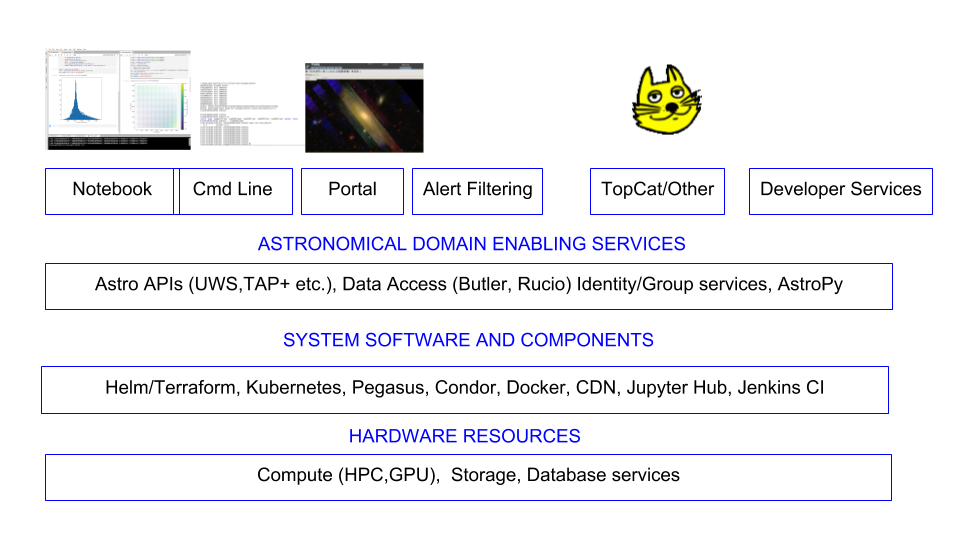
\includegraphics[width=0.45\textwidth]{CI-LSST}
\caption{Industry standard Cyber infrastructure model (left) and an astronomy instantiation of such a model (right)\label{fig:ci}}
\end{figure}

All funded funded astronomical projects with \emph{software deliverables leverage these APIs} for data access.
Of course this is not quite enough - the  \gls{API} layers must \emph{expose both data and \gls{metadata} in common
transferable and transformable formats} (e.g. \gls{CAOM}.

The astronomical community must develop \emph{data and \gls{metadata} transform services}
to support these common \gls{API} layers to aid interoperation. To further aid ease of use and cut down on wasted effort
all data providers should  to subscribe to a
\emph{common federated identity service} (e.g. InCommon or
Globus Auth) that is supported by most university and research organizations. There
must also be
an authentication source for users at institutions without such means and for
citizen science efforts.

This would imply that \emph{POSIX based file access be deprecated
in software development} and only used when applications require thread safe
data access (something that is currently not possible with \gls{FITS} files).

We should furthermore  develop a pseudo-directory structure system to
integrate local and remote files into a dynamic namespace for each user and potentially
each users use-case (e.g. the Box sync interface or the \gls{FUSE} based WholeTale file system
\citep{BRINCKMAN2019854})

\section{Why we should kill the filesystem}

Users should not care and repositories should not be tied to legacy formats  and storage representations because of legacy constraints  at other repositories.
The rest of the world has already moved on,  Google, Amazon, Git, netflix etc. do not host large filesystems and and can scale because they are not limited by this antiquated formalism.


Filesystems with name spaces are very fragile at large scale. As we get larger data sets we have to trick the filesystem to not run out of Inodes, we make countless sub directories to cope with our thousands of files.
This is turn leads to countless hours spent fighting over how to organize files  the \emph{right way} in a filesystem.
Countless years have been spent fighting over data formats (\gls{FITS} vs \gls{HDF} vs \gls{CSV} vs Pandas).
If we move code then perhaps the filesystem is not organised in the same manner and the code may not work - remote access to allow caching is not always an option.

We need to foster better remote collaboration.  The laptop is the bane of file sharing.
This has changed with cloud based pseudo-file systems but require storage in a single
cloud providers infrastructure. By creating a Filesystem as a Service (\gls{FSAAS}) federated
across data and cloud providers, we will win.


This "Infrastructure as Code" \citep{morris2016infrastructure} approach lowers the bar to entry
and allows for easier adoption of more standardized services that will enable large-scale
astronomical research in ways that are well demonstrated in plant genomics (CyVerse and Galaxy), natural hazards (Designsafe), and surface water research (Hydroshare).

\section{Example Service Architecture- The Butler}
The LSST butler

\section{Library example - AstroPy}
What is needed to go beyond \gls{LSST} and AstroPy?




% Include all the relevant bib files.
% https://lsst-texmf.lsst.io/lsstdoc.html#bibliographies
\bibliographystyle{yahapj}
\bibliography{local,lsst,lsst-dm,refs_ads,refs,books}

%Make sure lsst-texmf/bin/generateAcronyms.py is in your path
\printglossaries
\end{document}
